\documentclass[reprint,amsmath,amssymb,aps,prb]{revtex4-2}

\usepackage{graphicx}% Include figure files
\usepackage{dcolumn}% Align table columns on decimal point
\usepackage{bm}% bold math
\usepackage{hyperref}% add hypertext capabilities
\usepackage{xcolor}
\usepackage{braket}
\usepackage[english]{babel}

%% Philipps stuff %%
\usepackage{subcaption}
\captionsetup[subfigure]{list=true, font=large, labelfont=bf, 
	labelformat=brace, position=top}


%% Code stuff %%
\usepackage{listings} % insert code fragments

\definecolor{codegreen}{rgb}{0,0.6,0}
\definecolor{codegray}{rgb}{0.5,0.5,0.5}
\definecolor{codepurple}{rgb}{0.58,0,0.82}
\definecolor{backcolour}{rgb}{0.95,0.95,0.92}

\lstdefinestyle{mystyle}{
    backgroundcolor=\color{backcolour},   
    commentstyle=\color{codegreen},
    keywordstyle=\color{magenta},
    numberstyle=\tiny\color{codegray},
    stringstyle=\color{codepurple},
    basicstyle=\ttfamily\footnotesize,
    breakatwhitespace=false,         
    breaklines=true,                 
    captionpos=b,                    
    keepspaces=true,                 
    numbers=left,                    
    numbersep=5pt,                  
    showspaces=false,                
    showstringspaces=false,
    showtabs=false,                  
    tabsize=2
}

\lstset{style=mystyle}

\begin{document}

%\title{Project title}

\author{Your Name}

\date{\today}% It is always \today, today,
             %  but any date may be explicitly specified

\begin{abstract}
A paper usually includes an abstract, a concise summary of the work covered at length in the main body of the paper. Please also write a short abstract of your project.
\end{abstract}


\maketitle




\section{Guidelines}



Please write a short paper about your project. There are no strict length limits, but please write \textbf{at least two pages in the layout of this template} (including figures, excluding references and code listings). Please structure your paper in a scientific way, and include your references and your code. There are \LaTeX packages you can use to preserve the indentation of your code, e.g. the \texttt{listings} package which is demonstrated in the Appendix~\ref{app:codes}.

This sample document makes use of of REV\TeX~4.2, therefore you will need to install it to be able to compile this document yourself. Further information can be found in the REV\TeX~4.2
documentation included in the distribution or available at
\url{http://journals.aps.org/revtex/}.



\subsection{Example citations}
By default, citations are numerical\cite{epr}, some more citations~\cite{feyn54,Bire82,Berman1983,witten2001,Davies1998}. 

\subsection{Exampe figure}
Including and referring to figures is as usual, see for instance Fig.~\ref{fig:example}
\begin{figure}
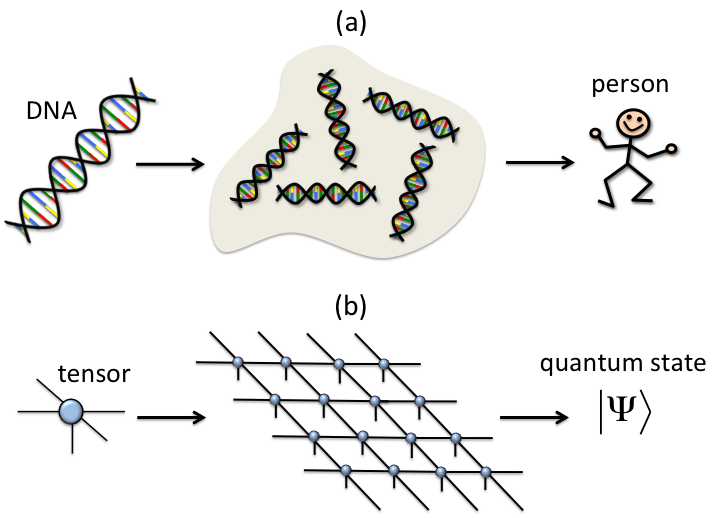
\includegraphics[width=0.99\linewidth]{cartoon.png}
\caption{Example of a figure~\cite{Orus2013}.}
\label{fig:example}
\end{figure}

\bibliography{bibsamp}% Produces the bibliography via BibTeX.


\appendix


\begin{widetext}
\section{Code listing} \label{app:codes}
Please copy your code in the appendix.
\begin{lstlisting}[language=Python]
"""

Module to generate the Hamiltonian of the transverse field Ising model.

H = -J sum_i sigma^x_i sigma^x_{i+1} - g sum_i sigma^z i.

Used in the solution of exercise 5.1

"""

import numpy as np
import scipy
from scipy import sparse
import scipy.sparse.linalg
import matplotlib.pyplot as plt

Id = sparse.csr_matrix(np.eye(2))
Sx = sparse.csr_matrix([[0., 1.], [1., 0.]])
Sz = sparse.csr_matrix([[1., 0.], [0., -1.]])
Splus = sparse.csr_matrix([[0., 1.], [0., 0.]])
Sminus = sparse.csr_matrix([[0., 0.], [1., 0.]])


def singesite_to_full(op, i, L):
    op_list = [Id]*L  # = [Id, Id, Id ...] with L entries
    op_list[i] = op
    full = op_list[0]
    for op_i in op_list[1:]:
        full = sparse.kron(full, op_i, format="csr")
    return full


def gen_sx_list(L):
    return [singesite_to_full(Sx, i, L) for i in range(L)]


def gen_sz_list(L):
    return [singesite_to_full(Sz, i, L) for i in range(L)]


def gen_hamiltonian_periodic(sx_list, sz_list, g, J=1.):
    """ assumes periodic boundery conditions """
    L = len(sx_list)
    H = sparse.csr_matrix((2**L, 2**L))
    for j in range(L):
        H = H - J *( sx_list[j] * sx_list[(j+1)%L])
        H = H - g * sz_list[j]
    return H
\end{lstlisting}
\end{widetext}

\title{Machine Learning of Many Body Localization}

\author{Philipp Krüger}

\date{\today}% It is always \today, today,
             %  but any date may be explicitly specified

\begin{abstract}
Exact diagonalization was used to find the reduced density matrices of the lowest energy eigenstate of the Heisenberg Model with an additional field in z-direction at low and high disorder strength. The resulting dataset representing extended and localized phases was used to train a neural network. Afterwards, the trained network was applied on intermediate disorder strengths to deduct the critical disorder strength for a phase transition. The phase transition occurred for all system sizes at $W_c = J$. 
%todo W-c is the same for all system sizes?
\end{abstract}

\maketitle

\section{Introduction}

Firstly, the physical model is introduced. Secondly, the concept of exact diagonalization is briefly presented. As we use the reduced density matrices as the feature for the neural network, we state briefly their derivation.
%Review Literature on task. How other people find $W_c$?
%Why is the topic interesting? => Finding Wc?
\subsection{Physical model}

\subsubsection{Hamiltonian of the Heisenberg model}

The hamiltonian of the Heisenberg model is shown in equation \ref{hamiltonian}. In the course of further analysis, we choose $J=1$ and sample $h$ from a uniform distribution such that $h_i \in \left[-W, W\right]$.

\begin{equation}
	H=\underbrace{J\sum_i \vec{S}_i\cdot\vec{S}_{i+1}}_{\text{Exchange Energy}}-\underbrace{\sum_ih_iS_i^z}_{\text{Random Field}}\label{hamiltonian}
\end{equation}

\subsubsection{Expectations for the ground state}

The expectation for the ground state is dependent on the ratio of the coupling and the local random field. 

For $\frac{W}{J} \ll 1$, we expect an extended, delocalized phase, since the exchange energy dominates over the small external field. Therefore, the system can relax to thermal equilibrium serving as its own heat bath in the limit of large system size $L\rightarrow\infty$.
Here, the reduced density operator of a finite subsystem converges to the equilibrium thermal distribution
for $L\rightarrow\infty$.\cite{Pal2010}

For $\frac{W}{J} \gg 1$, we can expect a localized phase, since the $h_i$ factors dominate over the exchange energy. The resulting states are expected to be product states of spins "up" or "down", as the external field points in z-direction. Also an infinite system cannot equilibrate itself. The local configurations are set by the initial conditions at all times and are adiabatically connected to the trivial state.\cite{Pal2010}

%non-thermalising phase, in which the system violates the Eigenstate Thermalisation hypothesis
%\url{https://arxiv.org/pdf/1610.03042.pdf}
%J<g: (large W) localized phase (), 

\subsection{Exact diagonalization}

Exact diagonalization (ED) is a numerical technique we can use to solve the Schrödinger Equation $H\ket{\psi}=E\ket{\psi}$ for the eigenvalues $E$ and eigenvectors $\ket{\psi}$. This only works of the Hamiltonian $H$ represents a discrete and finite system. Most quantum many-particle problems lead to a sparse matrix representation of the Hamiltonian, where only a very small fraction of the matrix
elements is non-zero.\cite{Weisse2008} A successful method can be found to find ground states is the Lanczos algorithm.\cite{Lanczos1950}

Introduce concepts: Exact Diagonalization,

\subsection{Areal (reduced??) Density Matrix}

areal Density Matrix:
\url{http://www.thphys.nuim.ie/staff/jvala/Lecture_9.pdf}

\begin{figure}[h!]
	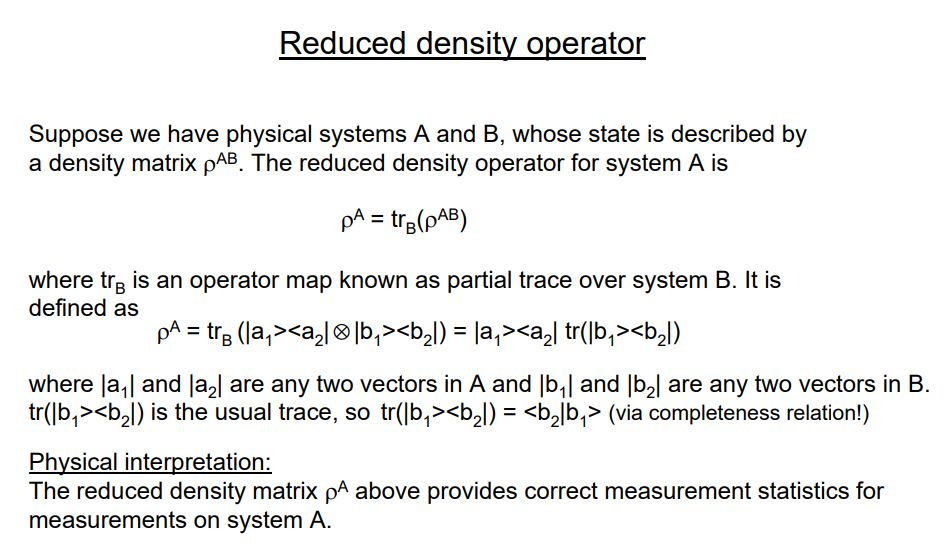
\includegraphics[width=0.99\linewidth]{figures/reduced_density_matrix.jpg}
	\caption{Example of a figure~\cite{Orus2013}.}
	\label{fig:adm}
\end{figure}

vs

direct density matrix:
(DOI: 10.1103/PhysRevB.99.054208 says 
Instead of dividing the system into two subsystems A
and B to calculate the reduced density matrix of an eigenstate rho a and using the entanglement spectrum as the training data set 34,35, we directly feed the
probability density of the eigenstate psi i computed in the
spin basis to the machines as the training data set. The
reason for doing so is that, although by preprocessing
the training data can reduce the dimension and filter out
redundant information, useful information contained in
the wavefunction of the entire system can also be lost.)

Conclusion: => areal

\subsection{Neural Networks and Convolutional Neural Networks}

Neural Network, CNN





\section{Materials and Methods}%todo: Action title

\subsection{Code Protocol}

\begin{enumerate}
	\item Function: Generate random disorder strength using a uniform distribution
	\item Function: Generate Hamiltonian from disorder strength and system size
	\item Define and understand phase transition from extended phase to localized phase
	\item Function: Picks a number M of lowest eigenstates near Energy E = 0
	\item Function: Generate density matrix for an eigenstate
	\item Function: Visualize density matrices
	\item  Function: Set up machine learning model that takes density matrices of different W as an input, 
	and predicts whether the state represents an extended or a localized phase.
	\item Function: Make predictions for different system sizes L and block sizes n.
	\item Function: Plot the predicitons over W.
	\item Function: Extract $W_c$
	from the data.
\end{enumerate}


Explain Flow with figure

\begin{figure}[h!]
	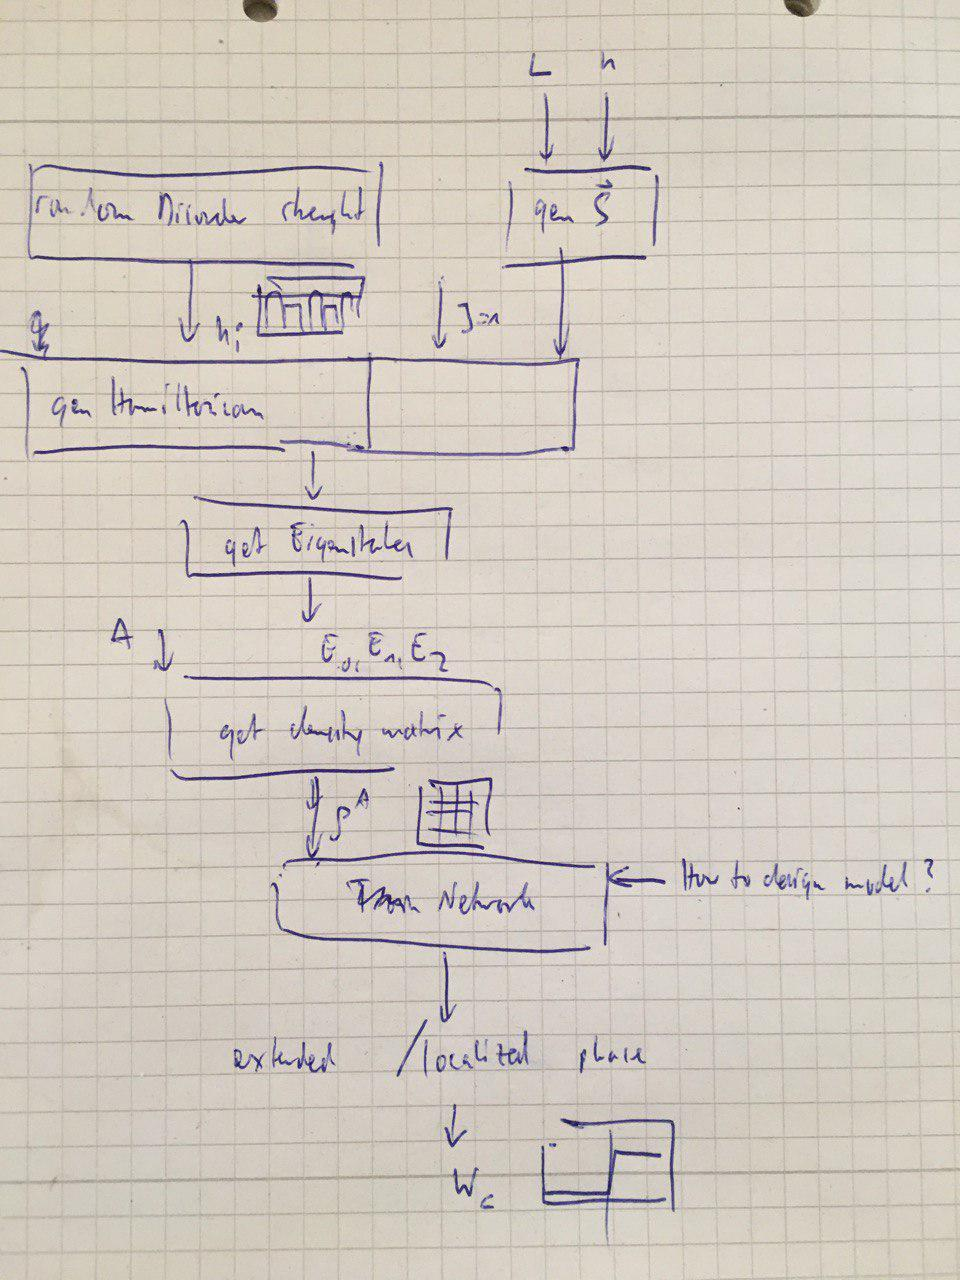
\includegraphics[width=0.99\linewidth]{figures/flowchart.jpg}
	\caption{Example of a figure~\cite{Orus2013}.}
	\label{fig:example}
\end{figure}

Fig.~\ref{fig:example}

\subsection{Machine Learning Models and Error Metrics}

Two different approaches:

regression like: Optimizer RMSprop, Loss MAE

classification focused: Optimizer Adam

Loss: BinaryCrossentropy from \url{https://keras.io/api/losses/probabilistic_losses/#binary_crossentropy-function}:
Computes the cross-entropy loss between true labels and predicted labels.

Use this cross-entropy loss when there are only two label classes (assumed to be 0 and 1). For each example, there should be a single floating-point value per prediction.

Optimizer: Stochastic Gradient Descent, Learning rate? Formula? Principle?

Explain metrics and errors and why they are used. Which ml models are used and why?

Use drop out to reduce overfitting. Low sample size techniques:

\section{Results}%todo: Action title

\subsection{Generation of density matrix training set}

Chosen parameters: $L \in \{10, 11, 12\}$. Repetitions: 500. Measure of variation in the test set??

\newpage
\begin{figure*}[h!]
	\begin{subfigure}[c]{0.3\textwidth}
		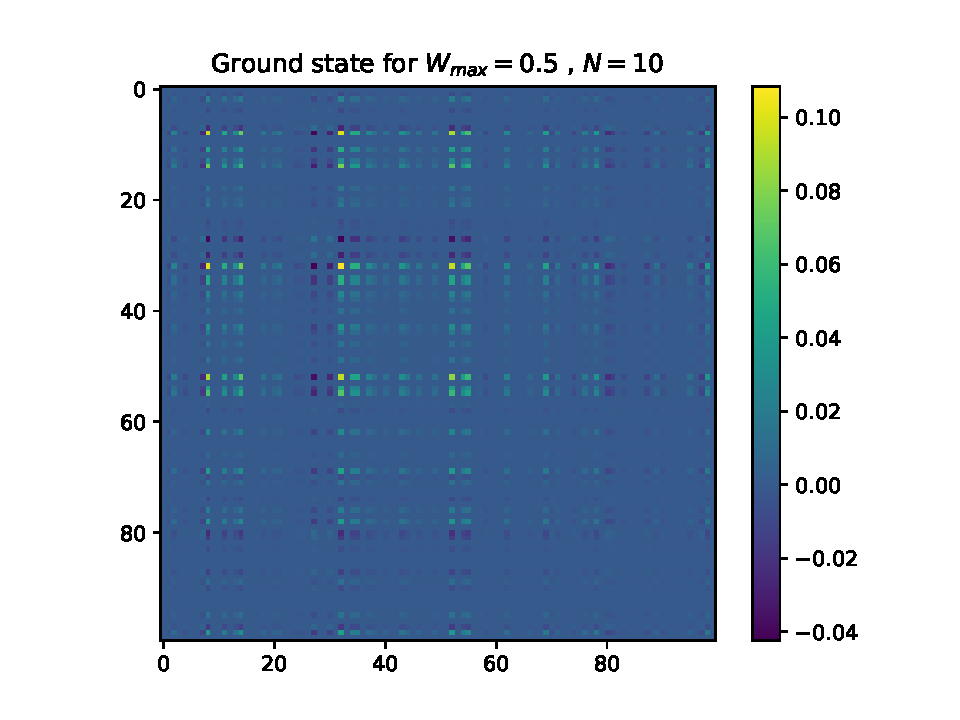
\includegraphics[width=\textwidth]{../results/N10_trainingset_groundstate_Wmax0.5.pdf}
		\subcaption{Ergodic phase L = 10.}
	\end{subfigure}
	\begin{subfigure}[c]{0.3\textwidth}
		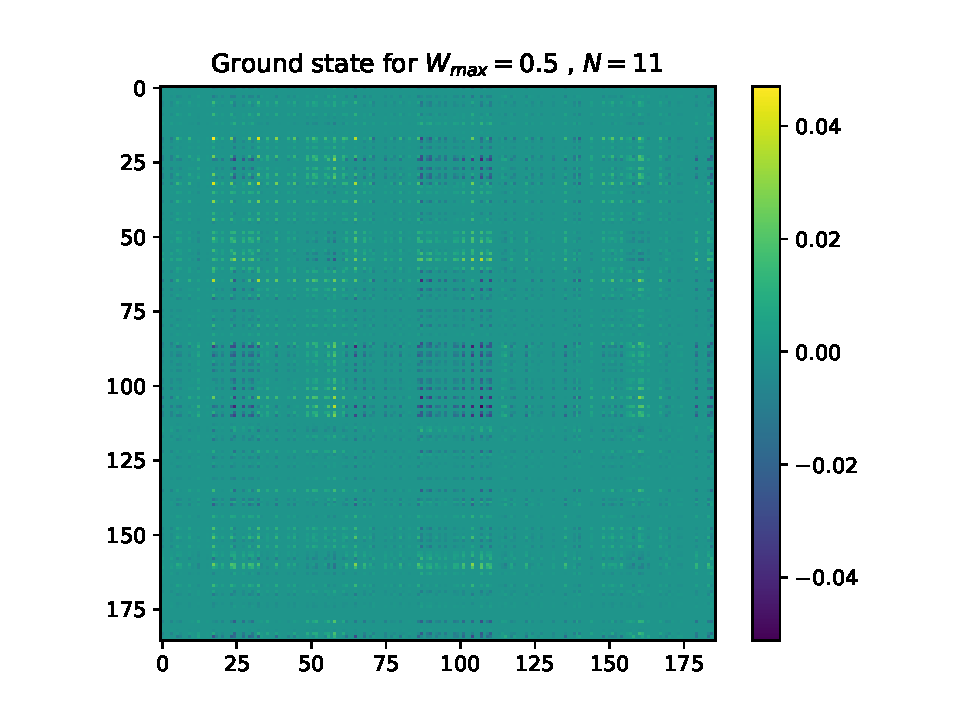
\includegraphics[width=\textwidth]{../results/N11_trainingset_groundstate_Wmax0.5.pdf}
		\subcaption{Ergodic phase L = 11.}
	\end{subfigure}
	\begin{subfigure}[c]{0.3\textwidth}
		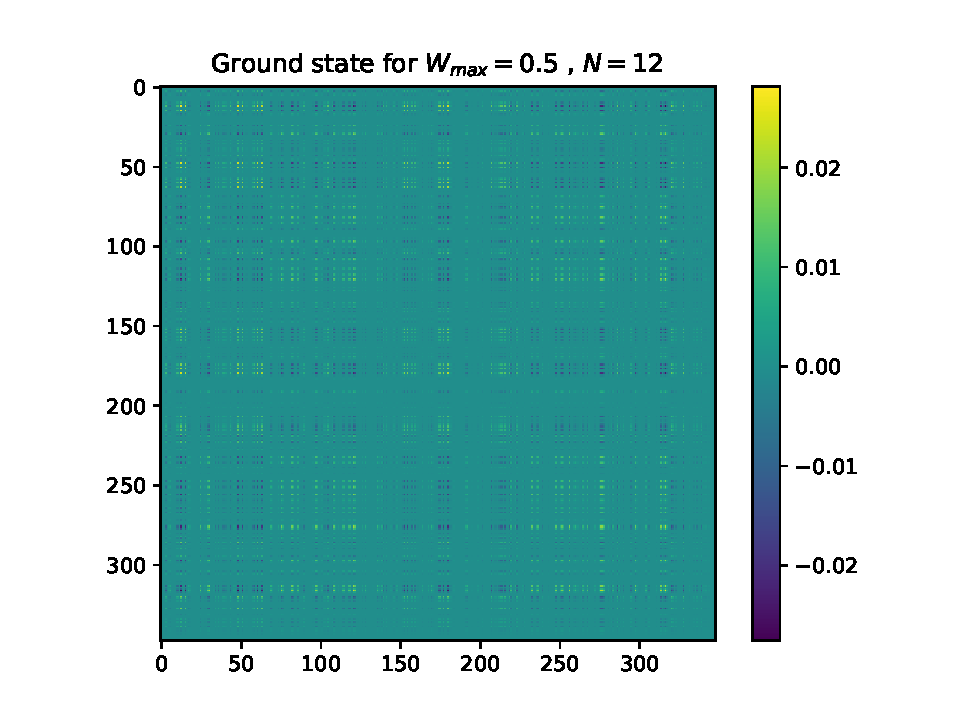
\includegraphics[width=\textwidth]{../results/N12_trainingset_groundstate_Wmax0.5.pdf}
		\subcaption{Ergodic phase L = 12.}
	\end{subfigure}
	\begin{subfigure}[c]{0.3\textwidth}
		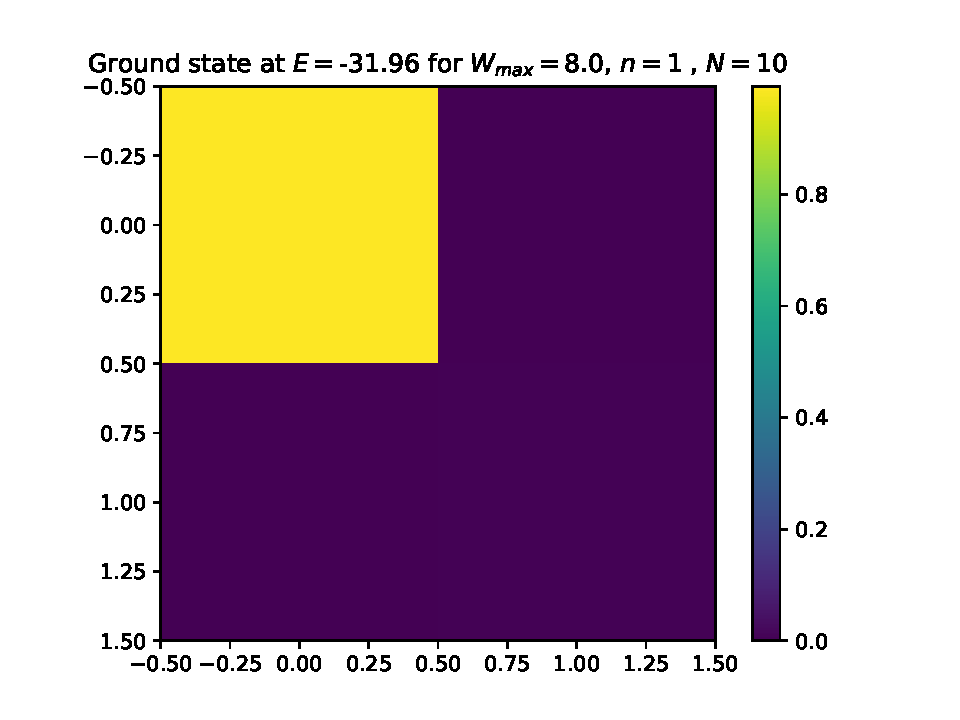
\includegraphics[width=\textwidth]{../results/N10_trainingset_groundstate_Wmax8.0.pdf}
		\subcaption{Localized phase L = 10.}
	\end{subfigure}
	\begin{subfigure}[c]{0.3\textwidth}
		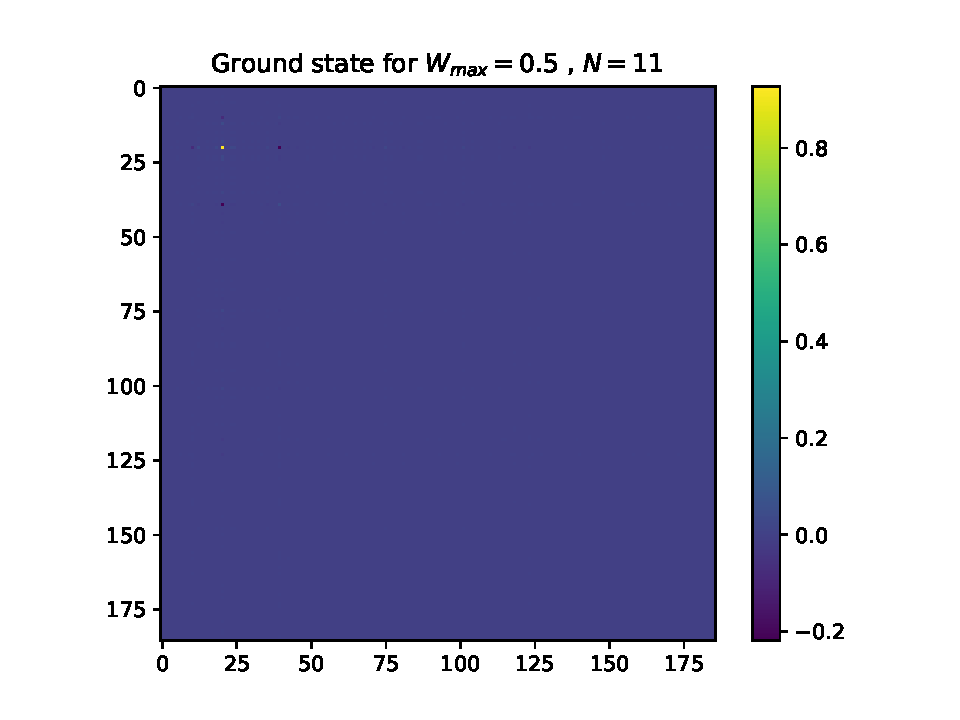
\includegraphics[width=\textwidth]{../results/N11_trainingset_groundstate_Wmax8.0.pdf}
		\subcaption{Localized phase L = 11.}
	\end{subfigure}
	\begin{subfigure}[c]{0.3\textwidth}
		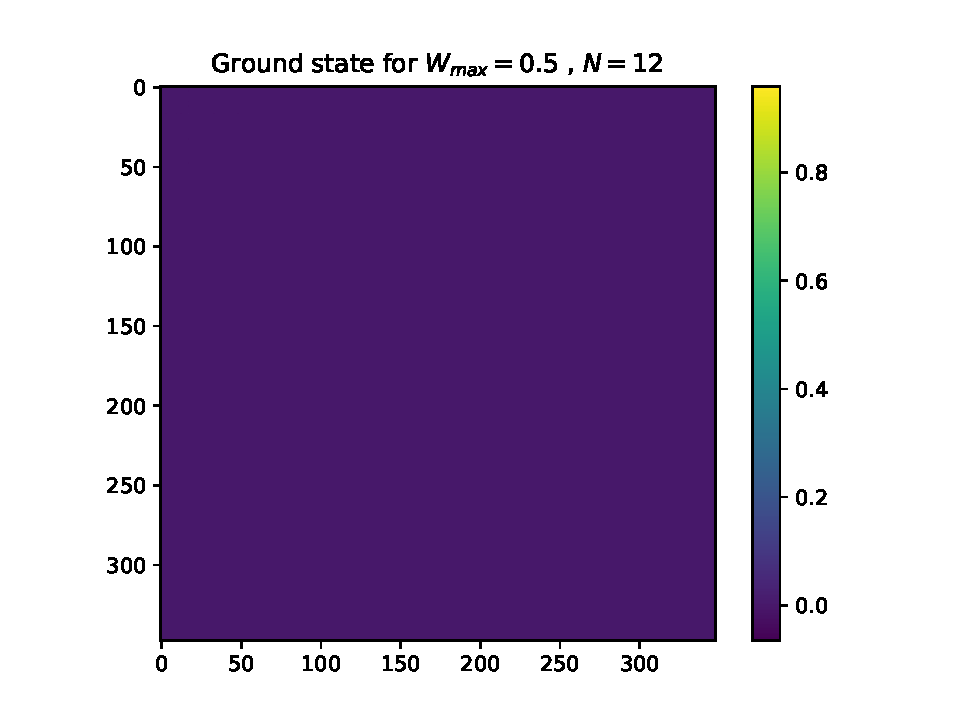
\includegraphics[width=\textwidth]{../results/N12_trainingset_groundstate_Wmax8.0.pdf}
		\subcaption{Localized phase L = 12.}
	\end{subfigure}
	\caption{Real part of the density matrix of an ergodic/localized phase for different system sizes L.}
\end{figure*}


%\begin{figure}
%	\begin{subfigure}[c]{0.2\textwidth}
%			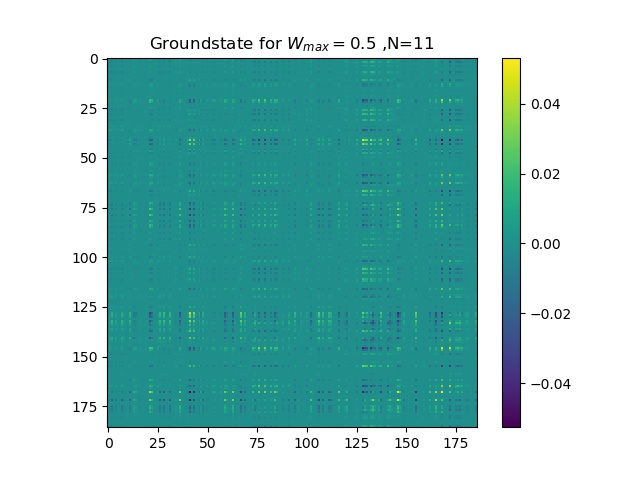
\includegraphics[width=\textwidth]{../results/N11_trainingset_groundstate_Wmax0.5.jpg}
%		\subcaption{}
%	\end{subfigure}
%	\begin{subfigure}[c]{0.2\textwidth}
%		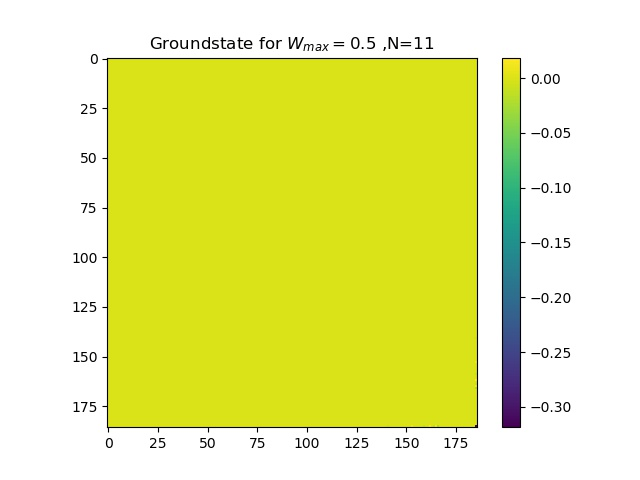
\includegraphics[width=\textwidth]{../results/N11_trainingset_groundstate_Wmax8.0.jpg}
%		\subcaption{}
%	\end{subfigure}
%	\caption{Zwei Bilder mit Subfigure nebeneinander}
%\end{figure}


Plots: 
What is computationally realizable in 1h concerning time?
The training set was sufficiently large enough 

We only need M Eigenstates

This is how corresponding density matrices look like

This will be our parameter space for n, L

\subsection{Prediction of extended vs localized phase}

Training and validation scores:

\newpage
\begin{figure*}[h!]
	\begin{subfigure}[c]{0.3\textwidth}
		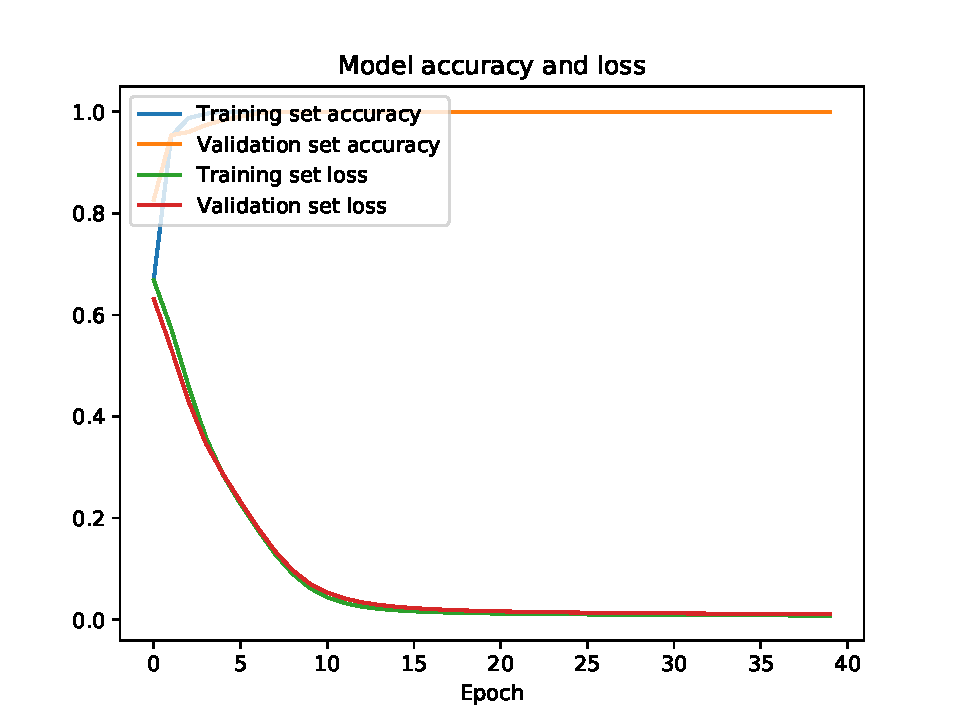
\includegraphics[width=\textwidth]{../results/N10_accuracy_loss_epochs}
		\subcaption{$N=10$}
		\label{fig:N10_accuracy_loss_epochs}
	\end{subfigure}
	\begin{subfigure}[c]{0.3\textwidth}
		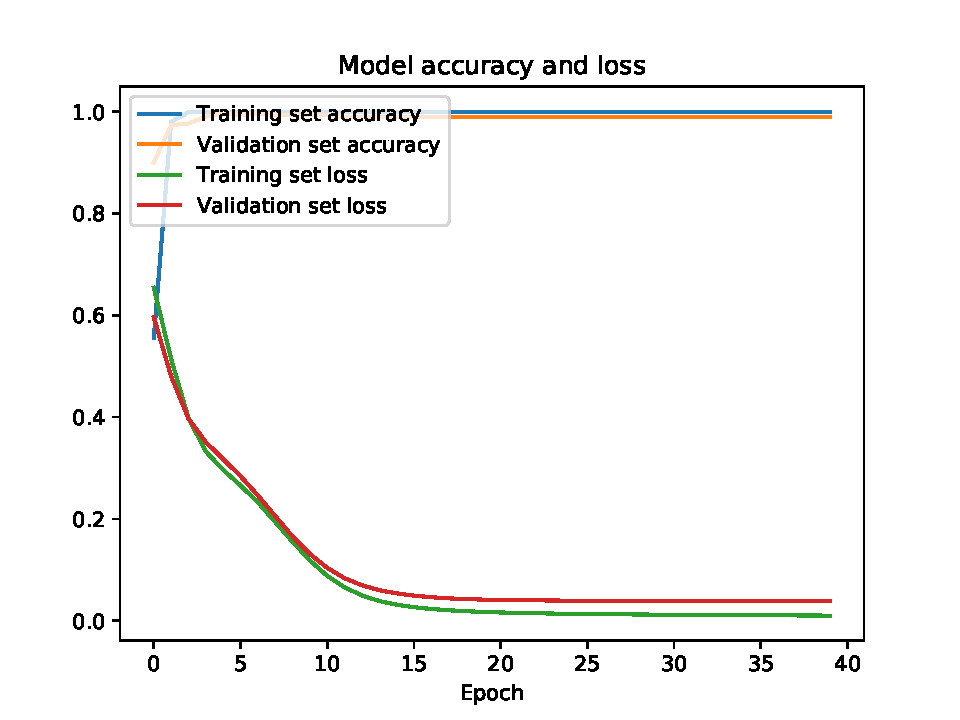
\includegraphics[width=\textwidth]{../results/N11_accuracy_loss_epochs}
		\subcaption{$N=11$}
		\label{fig:N11_loss_epochs}
	\end{subfigure}
	\begin{subfigure}[c]{0.3\textwidth}
		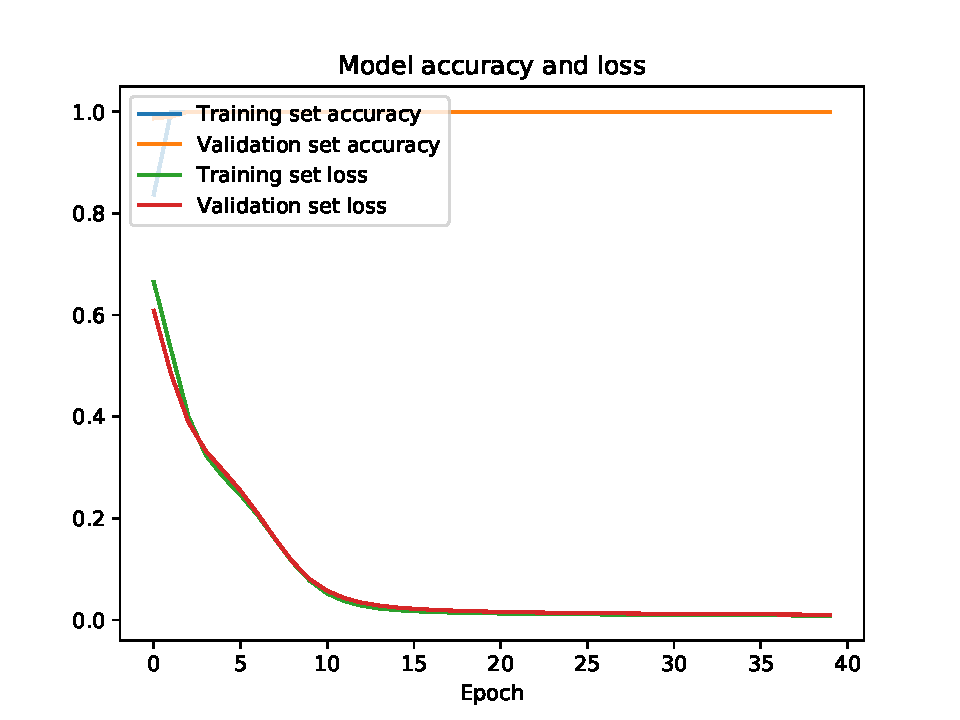
\includegraphics[width=\textwidth]{../results/N12_accuracy_loss_epochs}
		\subcaption{$N=12$}
		\label{fig:N12_loss_epochs}
	\end{subfigure}
	\caption{Accuracy and loss of neuronal network plotted over training epochs.}
\end{figure*}



\subsection{$W_c$ analysis}


Now we generate testing set with $W_{max} \in \left[0,4\right]$. We suspect $W_c$ to be at 1 ??%todo
We fit a logistic curve and extract $W_c$ as a parameter.

\newpage
\begin{figure*}[h!]
	\begin{subfigure}[c]{0.3\textwidth}
		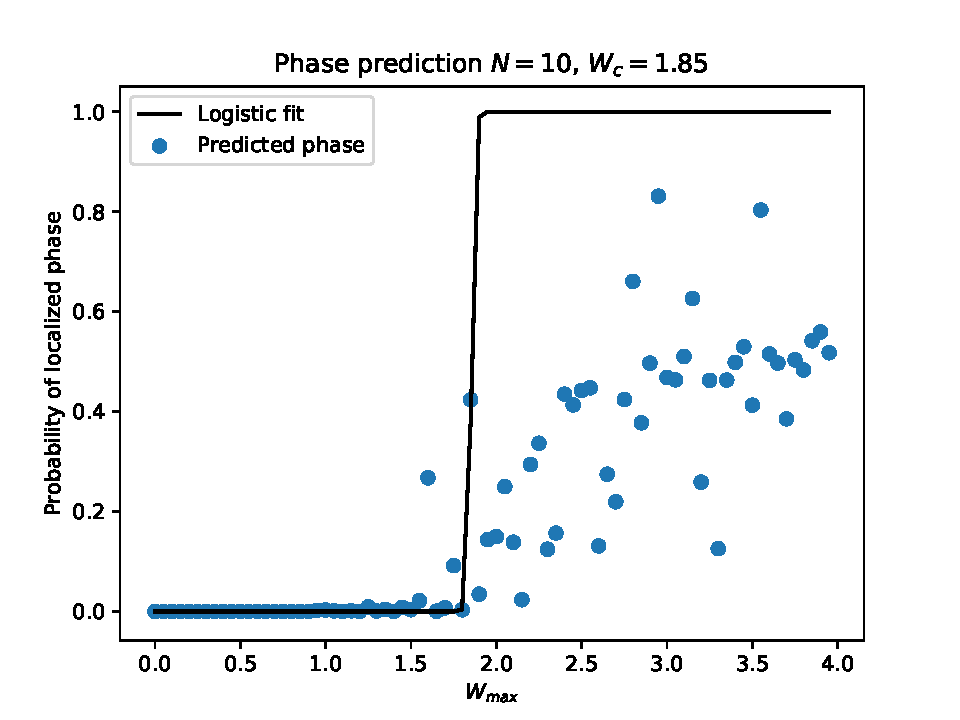
\includegraphics[width=\textwidth]{../results/N10_predict_wc}
		\subcaption{$N=10$}
		\label{fig:N10_predict_wc}
	\end{subfigure}
	\begin{subfigure}[c]{0.3\textwidth}
		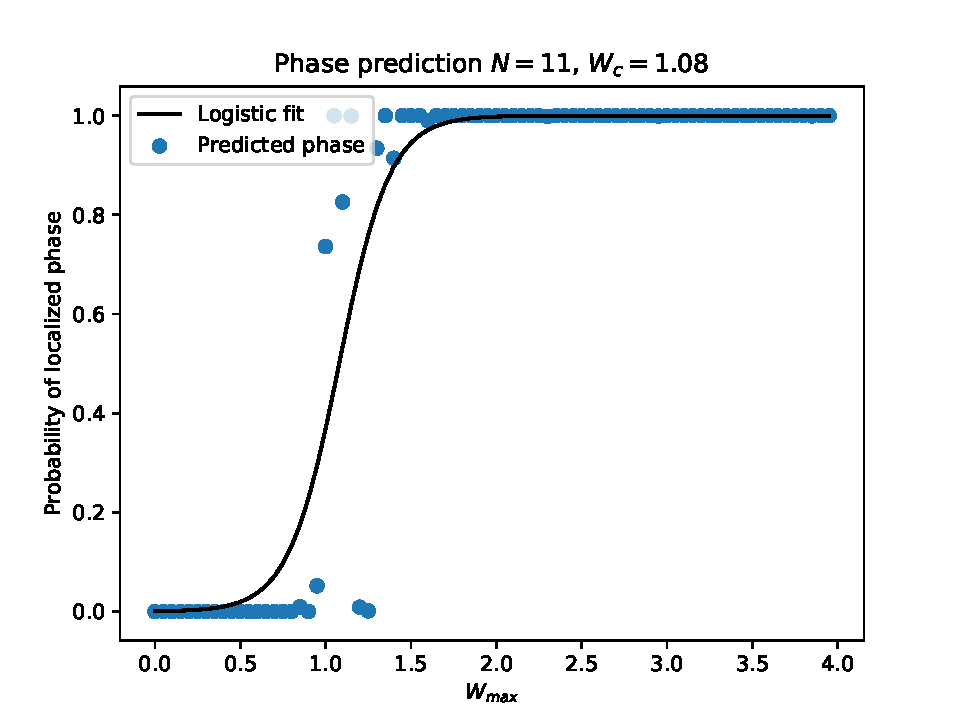
\includegraphics[width=\textwidth]{../results/N11_predict_wc}
		\subcaption{$N=11$}
		\label{fig:N11_predict_wc}
	\end{subfigure}
	\begin{subfigure}[c]{0.3\textwidth}
		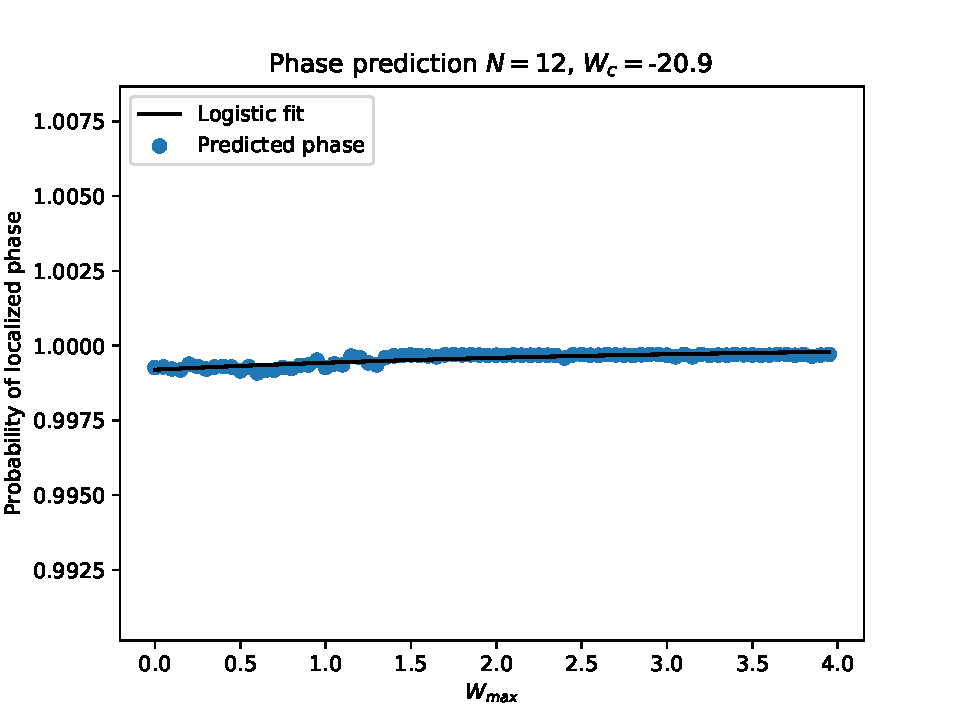
\includegraphics[width=\textwidth]{../results/N12_predict_wc}
		\subcaption{$N=12$}
		\label{fig:N12_predict_wc}
	\end{subfigure}
	\caption{Phase prediction with localized and ergodic phase defined as 1, 0.}
\end{figure*}


These are our $W_c$ depending on n, L.

%todo: Plot with extracted $W_Cs$

\begin{figure}
	\centering
	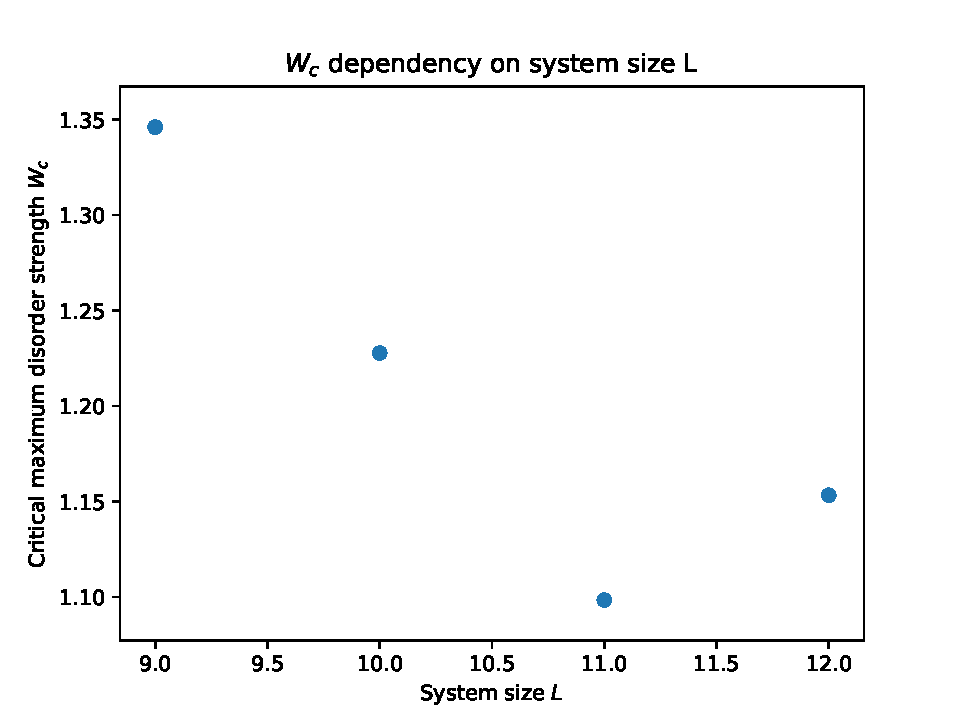
\includegraphics[width=0.7\linewidth]{../results/Wc_L_dependency}
	\caption{}
	\label{fig:Wc_L_dependency}
\end{figure}
\begin{figure}
\centering
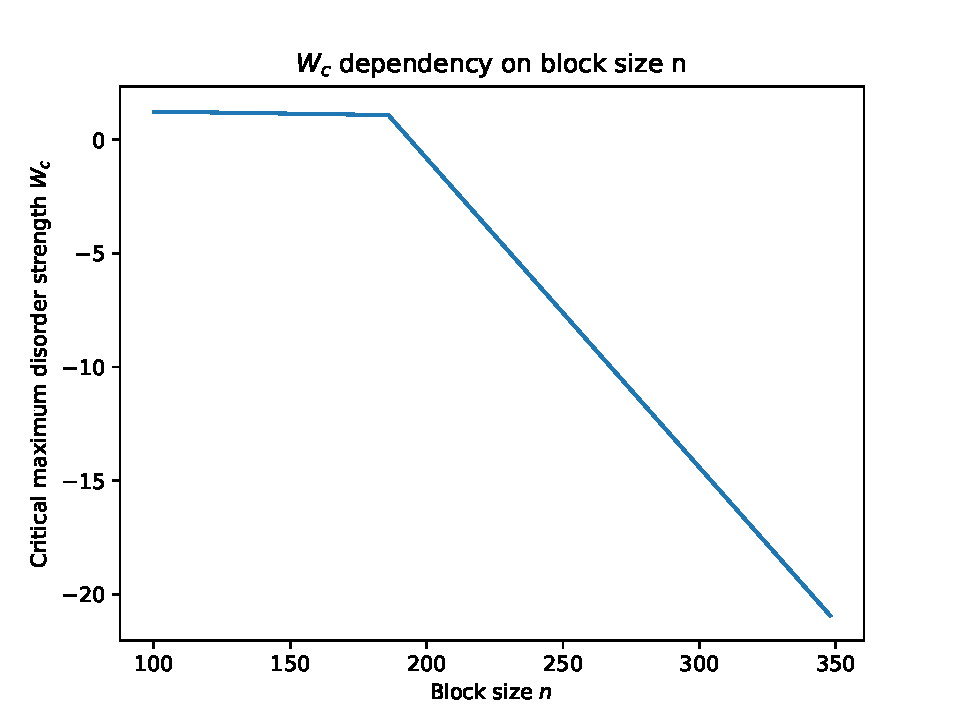
\includegraphics[width=0.7\linewidth]{../results/Wc_N_dependency}
\caption{}
\label{fig:Wc_N_dependency}
\end{figure}


\section{Conclusion}%todo: Action title

$W_c$ depends on n, L (yes/no).

$W_c$ prediction coincides with the expectation (yes/no)

$W_c$ is dependent on these and that effects => scaling analysis? (yes/no)

Citations are numerical\cite{epr}, some more citations~\cite{feyn54,Bire82,Berman1983,witten2001,Davies1998}. 

\bibliography{zotero}
%\bibliography{bibsamp}% Produces the bibliography via BibTeX.


\appendix


\begin{widetext}
\section{Code listing} \label{app:codes}
Please copy your code in the appendix.
\begin{lstlisting}[language=Python]
"""

Description

"""

import numpy as np

code
\end{lstlisting}
\end{widetext}



\end{document}
